% Template for Cogsci submission with R Markdown

% Stuff changed from original Markdown PLOS Template
\documentclass[10pt, letterpaper]{article}

\usepackage{cogsci}
\usepackage{pslatex}
\usepackage{float}
\usepackage{caption}

% amsmath package, useful for mathematical formulas
\usepackage{amsmath}

% amssymb package, useful for mathematical symbols
\usepackage{amssymb}

% hyperref package, useful for hyperlinks
\usepackage{hyperref}

% graphicx package, useful for including eps and pdf graphics
% include graphics with the command \includegraphics
\usepackage{graphicx}

% Sweave(-like)
\usepackage{fancyvrb}
\DefineVerbatimEnvironment{Sinput}{Verbatim}{fontshape=sl}
\DefineVerbatimEnvironment{Soutput}{Verbatim}{}
\DefineVerbatimEnvironment{Scode}{Verbatim}{fontshape=sl}
\newenvironment{Schunk}{}{}
\DefineVerbatimEnvironment{Code}{Verbatim}{}
\DefineVerbatimEnvironment{CodeInput}{Verbatim}{fontshape=sl}
\DefineVerbatimEnvironment{CodeOutput}{Verbatim}{}
\newenvironment{CodeChunk}{}{}

% cite package, to clean up citations in the main text. Do not remove.
\usepackage{apacite}

% KM added 1/4/18 to allow control of blind submission
\cogscifinalcopy

\usepackage{color}

% Use doublespacing - comment out for single spacing
%\usepackage{setspace}
%\doublespacing


% % Text layout
% \topmargin 0.0cm
% \oddsidemargin 0.5cm
% \evensidemargin 0.5cm
% \textwidth 16cm
% \textheight 21cm

\title{Identifying the distributional sources of children's early vocabulary}

\usepackage{booktabs}
\usepackage{longtable}
\usepackage{array}
\usepackage{multirow}
\usepackage{wrapfig}
\usepackage{float}
\usepackage{colortbl}
\usepackage{pdflscape}
\usepackage{tabu}
\usepackage{threeparttable}
\usepackage{threeparttablex}
\usepackage[normalem]{ulem}
\usepackage{makecell}
\usepackage{xcolor}

\author{{\large \bf George Kachergis*, Georgia Loukatou*, and Michael C. Frank } \AND {\large \bf  {kachergis, loukatou, mcfrank}@stanford.edu} \\  \newline\\ Department of Psychology, Stanford University, Stanford, CA 94305 USA\\ *equal contributions}


\begin{document}

\maketitle

\begin{abstract}
Children's early word learning is to a large extent driven by the
prevalence of words in their language environment, with words that are
spoken more often to children being learned earlier. However, children
receive language from a variety of sources, including books, television,
and movies meant for children, as well as speech and media that is meant
for adults, but overheard by children. Despite considerable similarity
of word frequency distributions from these different input sources,
there is also significant and predictable variability between them. For
example, function words are far more frequent in books than in everyday
speech, while early-learned nouns (e.g., `ball' and `mommy') are more
frequent in child-directed speech than in other sources. Children
receive a mixture of these different frequency distributions. The goal
of this paper is to better understand the shared and unique variance in
these input sources -- in both English and French -- and to evaluate how
predictive these distributions are of children's early word learning.

\textbf{Keywords:}
early language learning; CDI; vocabulary development; word frequency
distributions.
\end{abstract}

\hypertarget{introduction}{%
\section{Introduction}\label{introduction}}

How does speech addressed to children, heard on television, or read in
books impact the growth of children's early vocabulary? How does speech
from these sources relate to adult-directed sources of speech? And how
do these potential language sources combine with parental socio-economic
status (SES) to predict young children's vocabulary growth? Children
must learn words based on ambient linguistic input, and indeed the
amount of child-directed speech a child receives predicts later
vocabulary growth (Hart \& Risley, 1995). However, children's exposure
to different words can vary greatly depending on the source -- spoken
language vs.~books vs.~media -- and the register -- child-
vs.~adult-directed -- of the language. These input sources vary in word
frequency, as well as by various measures of quality. For example,
children's books have higher lexical diversity than child-directed
speech, and thus may represent an important source of lexical knowledge
(Montag, Jones, \& Smith, 2015). Moreover, the amount of input children
receive from these different input sources may vary from child to child,
which may account for some of the great variability seen in children's
early vocabulary growth (Fenson et al., 1994). Indeed, higher measures
of input quantity and quality have been found to relate to children's
faster vocabulary growth, and to often be related to parents' SES (Hoff,
2003; Rowe, 2012). SES is a composite concept and parental education has
often been used as the proxy of the parents' SES (see Rowe, 2018 as an
entry point to this literature). For example, Hoff (2003) compared the
speech of low versus high SES American mothers, with SES defined based
on education (college-educated versus high school).

Input word frequency varies significantly depending on the context.
Previous studies have shown that frequency matters for children's word
learning (for a review, see Ambridge, Kidd, Rowland, \& Theakston,
2015), and have observed an association between word frequency in
children's language environments and individual words' age of
acquisition (Goodman, Dale, \& Li, 2008). But word frequency in books is
not the same as frequency in conversational speech, with many function
words being far more frequent in books than in speech (Dawson, Hsiao,
Wei Ming Tan, Banerji, \& Nation, 2021; Montag et al., 2015).

Some differences between frequency distributions are intuitive:
``mommy'' is quite frequent in child-directed speech, yet not so common
in children's books, and even more rare in books meant for all ages. But
other differences are less intuitive: ``of'' is frequent in books meant
for all ages, and while still frequent in child-directed speech, it is
relatively less frequent as compared to children's books. In general,
speech -- whether directed to children or to adults -- contains
relatively fewer function words and tends to score lower on measures of
lexical diversity than books, which have a higher ratio of types (unique
words) per set of tokens (instances of words; Dawson et al., 2021).

In this paper, we have three primary research questions. Question 1: How
different are different input sources? We examine shared and unique
variance in word frequency across different sources of English and
French input, ranging from children's books and movies to child-directed
speech and even comparing to adult-directed books, movies, and speech.
Because of the substantial correlations between these different input
sources, we employ principal components analysis (PCA) as a way to
understand the relation between frequency distributions from different
sources and registers.

Question 2: What is the relation between input frequencies and
acquisition? We investigate how well these components predict English-
and French-learning children's early word learning, using aggregate
MacArthur-Bates Communicative Development Inventories (CDI) data from
Wordbank (Frank, Braginsky, Yurovsky, \& Marchman, 2017). CDIs include
parent-report checklists measuring children's early vocabulary, which
have proven to be reliable and valid indicators of children's growing
language skill (Fenson et al., 1994). Critically, CDI forms provide
information about \textgreater600 individual words that children
eventually learn to produce. These data allow us to investigate the role
of different frequency sources using the Age of Acquisition (AoA)
prediction paradigm, in which we use regression models to predict the
mean age (in months) at which 50\% of children are expected to know a
given CDI word (Braginsky, Yurovsky, Marchman, \& Frank, 2019; Goodman
et al., 2008).

Question 3: How do input frequencies relate to maternal education? An
intuitive hypothesis is that children of more highly-educated parents
may read more to their young children, although it should be noted that
parental education is strongly associated with household SES--to the
extent that the former is often used as a proxy for the latter. Indeed,
young children from higher-SES households tend to have larger vocabulary
(Fernald, Marchman, \& Weisleder, 2013), and parents with higher-SES
tend to report reading more to their young children than parents with
lower SES. Thus, we test which sources of input frequency combine with
maternal education to better predict children's acquisition of
particular words, expecting that we may see evidence of earlier learning
of words from children's books in households with higher maternal
education (and SES).

Together, the answers to these questions provide insight into whether
word frequency acts as a single factor in vocabulary learning, or
whether different sources and registers have distinguishable effects.

\hypertarget{method}{%
\section{Method}\label{method}}

\hypertarget{datasets}{%
\subsection{Datasets}\label{datasets}}

We used corpora from different sources to identify shared and distinct
variance in frequencies. These corpora vary widely in size due to data
accessibility; several were created for the current study and are
available in our GitHub repository, together with all analysis scripts.

\begin{CodeChunk}
\begin{figure}[t]

{\centering 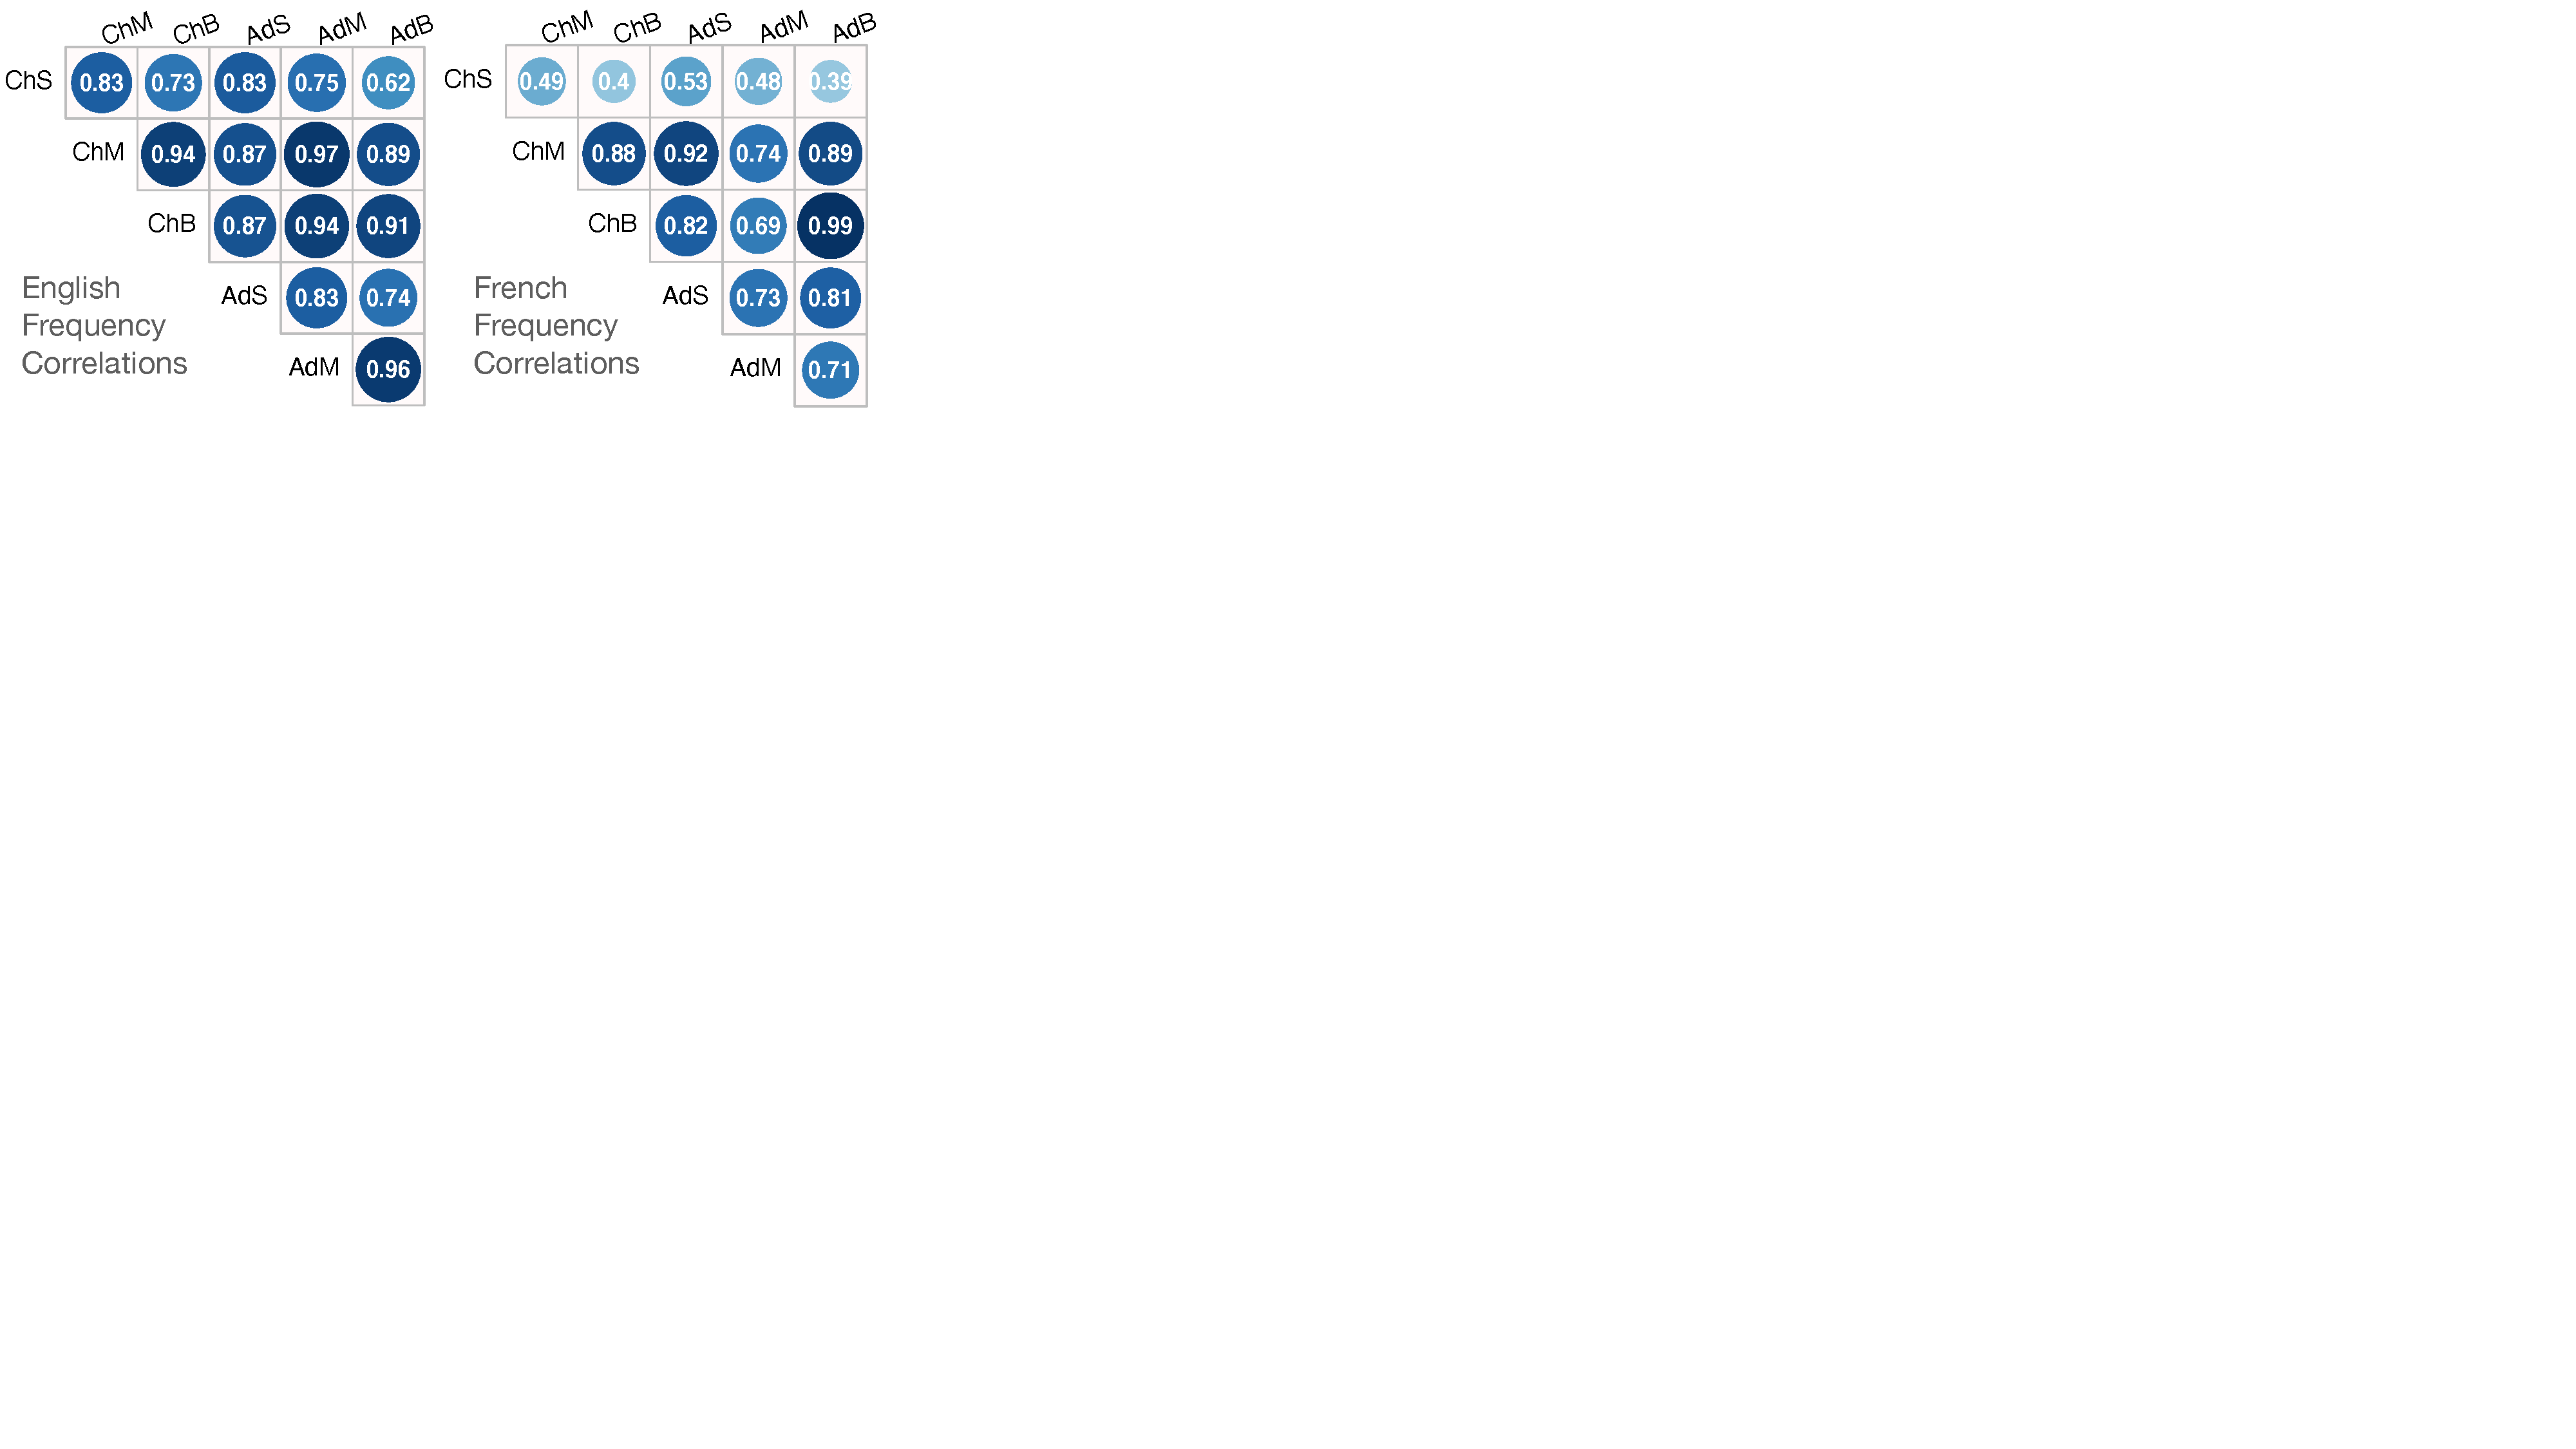
\includegraphics[width=\linewidth]{figs/corpus_freq_cors_hor} 

}

\caption[Word frequency correlations between different corpus sources for the CDI words in English and French]{Word frequency correlations between different corpus sources for the CDI words in English and French.}\label{fig:fig1}
\end{figure}
\end{CodeChunk}

\hypertarget{child-directed-speech-chs.}{%
\subsubsection{Child-directed Speech
(ChS).}\label{child-directed-speech-chs.}}

Utterances of ChS were extracted from CHILDES (MacWhinney (2000);
excluding book reading corpora), a collection of transcripts of
interactions between caregivers and children 0 to 12 years of age
(\(M=2.9\) years). After cleaning, the CHILDES English corpus yielded
5521000 tokens across 38779 word types. The French ChS yielded 3190000
tokens across 13139 word types.

\hypertarget{child-directed-books-chb.}{%
\subsubsection{Child-directed books
(ChB).}\label{child-directed-books-chb.}}

We used a sample of 98 English children's books from Project Gutenberg's
open-source database, previously used in machine learning research on
language comprehension (Hill, Bordes, Chopra, \& Weston, 2015). The
books were published between 1820 and 1922, but include well-known
titles as \emph{The Legend of Sleepy Hollow}. We also used 130 popular
French children stories accessible in parenting websites
(\url{https://fr.hellokids.com/}) and 10 French children books from
Project Gutenberg. After cleaning, the English ChB corpus totals 4673000
tokens across 42444 word types, and the French ChB totals 1298000 tokens
across 17990 word types.

\hypertarget{child-directed-media-chm.}{%
\subsubsection{Child-directed Media
(ChM).}\label{child-directed-media-chm.}}

Transcripts were extracted from English television shows (e.g., from PBS
Kids and Nickelodeon) and movies (e.g., \emph{Beauty and the Beast}),
including 1,078 movies and 4,309 TV episodes taken from Charlesworth,
Yang, Mann, Kurdi, \& Banaji (2021) (available here:
\url{https://osf.io/kqux5/}. Openly accessible transcripts
(\url{https://www.subsynchro.com/}) were also extracted from 100 French
films directed to children. After cleaning, the English ChM totals
6724000 tokens across 80082 word types. The French ChM totals 842000
tokens across 14937 word types.

\hypertarget{adult-directed-speech-ads.}{%
\subsubsection{Adult-directed Speech
(AdS).}\label{adult-directed-speech-ads.}}

English AdS was obtained from the Switchboard-1 Telephone Speech Corpus
(Godfrey \& Holliman, 1993), a corpus of transcripts from approximately
2,400 dyadic telephone conversations. After cleaning, the English AdS
yielded 3104000 tokens across 27479 word types. French AdS was obtained
from the TCOF corpus (André \& Canut, 2010), the CLAPI corpus (Balthasar
\& Bert, 2005) and the CFPP corpus (Branca-Rosoff, Fleury, Lefeuvre, \&
Pires, 2012). The French AdS yielded 1466000 tokens across 14486 word
types.

\hypertarget{adult-directed-books-adb.}{%
\subsubsection{Adult-directed Books
(AdB).}\label{adult-directed-books-adb.}}

The English AdB corpus is taken from a sample of 1,000 Project Gutenberg
books tokens randomly selected by Charlesworth et al. (2021), totaling
40252700 tokens across 147937 word types. The French AdB is comprised of
books taken from the 1999 Association de Bibliophiles Universels, an
open-source database of french books. After cleaning, it yielded 2288000
tokens across 30615 word types.

\hypertarget{adult-directed-media-adm.}{%
\subsubsection{Adult-directed Media
(AdM).}\label{adult-directed-media-adm.}}

The English AdM is comprised of 6060000 tokens across 60626 word types
compiled by Charlesworth et al. (2021) from online transcripts of movies
and TV shows dating from the 1960s (e.g., \emph{Doctor Who}) through the
present (e.g., \emph{Breaking Bad}). The French AdM corpus is comprised
of 767000 tokens across 15635 word types, after cleaning openly
accessible movie subtitles (\url{https://www.subsynchro.com/}) from 100
films.

\hypertarget{age-of-acquisition-data}{%
\subsubsection{Age of Acquisition data}\label{age-of-acquisition-data}}

Children's early word learning data was drawn from the CDIs (Fenson et
al., 2007), aggregated in the Wordbank database (Frank et al., 2017)
(data from 5520 children aged 16-30 months for the American English CDI:
Words \& Sentences (WS) form, and 641 children for the French French
CDI:WS form). Age of acquisition estimates were calculated via the
Wordbankr package. We computed the proportion of children at each age
who were reported to produce each word on the CDI forms completed by
parents. We then fit a curve to these proportions using a logistic
regression model and determined when the predicted acquisition curve
crossed 0.5 (when at least 50\% of children are reported to produce the
word).

\hypertarget{merging-the-corpora}{%
\subsection{Merging the Corpora}\label{merging-the-corpora}}

We focus our analysis on the 670 words from the English CDI and 632
words from the French CDI that were present in at least one of the
corpora. For French, because of the presence of more complex morphology,
CDI words were matched to related words in corpora via a stemmer
(Porter, 2001). All word frequencies were normalized to number of tokens
per million (TPM). For any CDI words that failed to appear in a given
corpus, we replaced the missing word's frequency with a normalized count
of 10 TPM, or the minimum normalized frequency for that distribution,
whichever was smaller.\footnote{Other forms of smoothing, e.g.~Laplace
  smoothing (\(\alpha=10\); added to all counts, including missing
  words) yielded similar results.}

\hypertarget{results}{%
\section{Results}\label{results}}

\hypertarget{cross-corpus-frequency-correlations-q1}{%
\subsection{Cross-corpus Frequency Correlations
(Q1)}\label{cross-corpus-frequency-correlations-q1}}

Figure 1 shows the word frequency correlations between different corpus
sources ({[}Adult- vs.~Child-directed{]} x {[}Speech, Books, Media{]})
for the matched CDI words (left: English, right: French).
Unsurprisingly, there were strong correlations across these different
corpora, but correlations were stronger within register and within
source for both English and French. Overall, French distributions were
more highly correlated with one another, likely due to smaller corpus
sizes.\footnote{The French corpora had a large number of CDI words
  missing (and thus smoothed): 95 in AdB; 77 in AdS; 70 in AdM; 99 in
  ChB; 12 in ChS; 53 in ChM. In comparison, English had 1 missing in
  ChB, ChS, and ChM; 14 in Adb; 45 in AdS; 28 in AdM.}

We used principal components analysis to disentangle these correlated
distributions and to understand their relationship. PCA allows us to
project word frequencies into a space in which the first dimension
captures the shared variance between frequencies from different sources
and registers, and subsequent dimensions capture other consistent
sources of variation. Since the logarithm of frequency is typically used
as a psycholinguistic predictor in previous studies (Braginsky et al.,
2019; Goodman et al., 2008), we perform our PCAs over log frequencies.
The eigenvectors of the PCs in relation to the original six frequency
distributions are summarized for English in Table 1, and for French in
Table 2, along with the proportion of variance (PVar) explained by each
component. PC1 already explains the bulk of the variance (89\% for
English and 90.2\% for French); and PC2-PC4 each only capture an
additional 2-4\% of the variance for both languages.

Table 3 provides qualitative descriptions of the principal components
(PC1-PC6) for each language. Note that the signs of eigenvectors in PCA
are arbitrary, so on some PCs positive values correspond to higher
absolute frequencies, while on others negative values correspond to
higher absolute frequencies. The first PC is similar for both English
and French, and captures shared variance between all frequency sources
and registers, representing words that are high or low frequency across
them. This means that frequency distributions are largely similar across
sources and registers. For English, the PCs align surprisingly well with
particular dimensions of the English frequency distributions: PC1 with
overall frequency, PC2 with child-directed speech, PC3 with
adult-directed speech, PC4 with media vs.~books, PC5 with child-directed
books vs.~speech, and PC6 with adult- vs.~child-directed media. For
French, we observe a similar pattern of findings. A difference lies on
PC2; it mostly captures child-directed speech for English, whereas for
French it captures book language.

\begin{CodeChunk}
\begin{table}

\caption{\label{tab:pca-en-table}English PC rotations and proportion of variance (PVar), colored by value (low=black; high=orange).}
\centering
\begin{tabular}[t]{>{}l>{}r>{}r>{}r>{}r>{}r>{}r}
\toprule
  & PC1 & PC2 & PC3 & PC4 & PC5 & PC6\\
\midrule
\cellcolor{white}{\textcolor{black}{ChM}} & \cellcolor[HTML]{1B1043}{\textcolor{white}{\em{-0.31}}} & \cellcolor[HTML]{A02F7F}{\textcolor{white}{0.15}} & \cellcolor[HTML]{000004}{\textcolor{white}{\textbf{-0.34}}} & \cellcolor[HTML]{FB835F}{\textcolor{white}{0.40}} & \cellcolor[HTML]{E44F64}{\textcolor{white}{0.28}} & \cellcolor[HTML]{FE9F6D}{\textcolor{white}{\textbf{0.73}}}\\
\cellcolor{white}{\textcolor{black}{ChB}} & \cellcolor[HTML]{150E37}{\textcolor{white}{\em{-0.34}}} & \cellcolor[HTML]{BB3978}{\textcolor{white}{0.25}} & \cellcolor[HTML]{020109}{\textcolor{white}{-0.32}} & \cellcolor[HTML]{000004}{\textcolor{white}{-0.63}} & \cellcolor[HTML]{FE9F6D}{\textcolor{white}{\textbf{0.53}}} & \cellcolor[HTML]{3D0F71}{\textcolor{white}{-0.21}}\\
\cellcolor{white}{\textcolor{black}{ChS}} & \cellcolor[HTML]{251254}{\textcolor{white}{\em{-0.26}}} & \cellcolor[HTML]{FE9F6D}{\textcolor{white}{\textbf{0.65}}} & \cellcolor[HTML]{030312}{\textcolor{white}{-0.30}} & \cellcolor[HTML]{C53C74}{\textcolor{white}{0.12}} & \cellcolor[HTML]{000004}{\textcolor{white}{\textbf{-0.60}}} & \cellcolor[HTML]{38106C}{\textcolor{white}{-0.22}}\\
\cellcolor{white}{\textcolor{black}{AdM}} & \cellcolor[HTML]{030310}{\textcolor{white}{\em{-0.47}}} & \cellcolor[HTML]{02020B}{\textcolor{white}{-0.45}} & \cellcolor[HTML]{0D0A29}{\textcolor{white}{-0.24}} & \cellcolor[HTML]{FE9F6D}{\textcolor{white}{\textbf{0.48}}} & \cellcolor[HTML]{BC3978}{\textcolor{white}{0.13}} & \cellcolor[HTML]{000004}{\textcolor{white}{\textbf{-0.53}}}\\
\cellcolor{white}{\textcolor{black}{AdB}} & \cellcolor[HTML]{020109}{\textcolor{white}{\em{-0.49}}} & \cellcolor[HTML]{000004}{\textcolor{white}{\textbf{-0.47}}} & \cellcolor[HTML]{491078}{\textcolor{white}{-0.01}} & \cellcolor[HTML]{21114E}{\textcolor{white}{-0.44}} & \cellcolor[HTML]{0C0927}{\textcolor{white}{-0.50}} & \cellcolor[HTML]{C63C73}{\textcolor{white}{0.32}}\\
\addlinespace
\cellcolor{white}{\textcolor{black}{AdS}} & \cellcolor[HTML]{000004}{\textcolor{white}{\em{-0.52}}} & \cellcolor[HTML]{C23B75}{\textcolor{white}{0.27}} & \cellcolor[HTML]{FE9F6D}{\textcolor{white}{\textbf{0.79}}} & \cellcolor[HTML]{C13A75}{\textcolor{white}{0.10}} & \cellcolor[HTML]{C03A77}{\textcolor{white}{0.14}} & \cellcolor[HTML]{721F81}{\textcolor{white}{-0.01}}\\
\cellcolor{white}{\textcolor{black}{PVar}} & \cellcolor{white}{\textcolor{black}{0.89}} & \cellcolor{white}{\textcolor{black}{0.04}} & \cellcolor{white}{\textcolor{black}{0.03}} & \cellcolor{white}{\textcolor{black}{0.02}} & \cellcolor{white}{\textcolor{black}{0.01}} & \cellcolor{white}{\textcolor{black}{0.01}}\\
\bottomrule
\end{tabular}
\end{table}

\end{CodeChunk}

\begin{CodeChunk}
\begin{table}

\caption{\label{tab:pca-fr-table}French principal component rotations.}
\centering
\begin{tabular}[t]{>{}l>{}r>{}r>{}r>{}r>{}r>{}r}
\toprule
  & PC1 & PC2 & PC3 & PC4 & PC5 & PC6\\
\midrule
\cellcolor{white}{\textcolor{black}{ChM}} & \cellcolor[HTML]{010107}{\textcolor{white}{\em{-0.41}}} & \cellcolor[HTML]{6A1C81}{\textcolor{white}{-0.09}} & \cellcolor[HTML]{852781}{\textcolor{white}{0.06}} & \cellcolor[HTML]{000004}{\textcolor{white}{\textbf{-0.65}}} & \cellcolor[HTML]{FE9F6D}{\textcolor{white}{\textbf{0.54}}} & \cellcolor[HTML]{E04C67}{\textcolor{white}{0.32}}\\
\cellcolor{white}{\textcolor{black}{ChB}} & \cellcolor[HTML]{010105}{\textcolor{white}{\em{-0.41}}} & \cellcolor[HTML]{FE9F6D}{\textcolor{white}{\textbf{0.55}}} & \cellcolor[HTML]{A8327D}{\textcolor{white}{0.20}} & \cellcolor[HTML]{BF3A77}{\textcolor{white}{0.13}} & \cellcolor[HTML]{E34E65}{\textcolor{white}{0.28}} & \cellcolor[HTML]{000004}{\textcolor{white}{\textbf{-0.63}}}\\
\cellcolor{white}{\textcolor{black}{ChS}} & \cellcolor[HTML]{050415}{\textcolor{white}{\em{-0.36}}} & \cellcolor[HTML]{000004}{\textcolor{white}{\textbf{-0.50}}} & \cellcolor[HTML]{FE9F6D}{\textcolor{white}{\textbf{0.73}}} & \cellcolor[HTML]{DC4869}{\textcolor{white}{0.24}} & \cellcolor[HTML]{6A1C81}{\textcolor{white}{-0.16}} & \cellcolor[HTML]{922B80}{\textcolor{white}{0.01}}\\
\cellcolor{white}{\textcolor{black}{AdM}} & \cellcolor[HTML]{000004}{\textcolor{white}{\em{-0.42}}} & \cellcolor[HTML]{491078}{\textcolor{white}{-0.19}} & \cellcolor[HTML]{21114E}{\textcolor{white}{-0.33}} & \cellcolor[HTML]{29115A}{\textcolor{white}{-0.42}} & \cellcolor[HTML]{000004}{\textcolor{white}{\textbf{-0.61}}} & \cellcolor[HTML]{331068}{\textcolor{white}{-0.35}}\\
\cellcolor{white}{\textcolor{black}{AdB}} & \cellcolor[HTML]{010107}{\textcolor{white}{\em{-0.41}}} & \cellcolor[HTML]{FD9C6B}{\textcolor{white}{\textbf{0.54}}} & \cellcolor[HTML]{7A2282}{\textcolor{white}{0.01}} & \cellcolor[HTML]{CD4071}{\textcolor{white}{0.18}} & \cellcolor[HTML]{2F1163}{\textcolor{white}{-0.36}} & \cellcolor[HTML]{FE9F6D}{\textcolor{white}{\textbf{0.62}}}\\
\addlinespace
\cellcolor{white}{\textcolor{black}{AdS}} & \cellcolor[HTML]{000004}{\textcolor{white}{\em{-0.42}}} & \cellcolor[HTML]{1B1043}{\textcolor{white}{-0.34}} & \cellcolor[HTML]{000004}{\textcolor{white}{\textbf{-0.56}}} & \cellcolor[HTML]{FE9F6D}{\textcolor{white}{\textbf{0.54}}} & \cellcolor[HTML]{E95362}{\textcolor{white}{0.30}} & \cellcolor[HTML]{9C2E7F}{\textcolor{white}{0.05}}\\
\cellcolor{white}{\textcolor{black}{PVar}} & \cellcolor{white}{\textcolor{black}{0.90}} & \cellcolor{white}{\textcolor{black}{0.04}} & \cellcolor{white}{\textcolor{black}{0.03}} & \cellcolor{white}{\textcolor{black}{0.02}} & \cellcolor{white}{\textcolor{black}{0.01}} & \cellcolor{white}{\textcolor{black}{0.00}}\\
\bottomrule
\end{tabular}
\end{table}

\end{CodeChunk}

\begin{CodeChunk}



\begin{table}[tbp]

\begin{center}
\begin{threeparttable}

\caption{\label{tab:table3}English (EN) \& French (FR) PC descriptions.}

\begin{tabular}{lllll}
\toprule
Lang & \multicolumn{1}{c}{PC} & \multicolumn{1}{c}{Description} & \multicolumn{1}{c}{Highest} & \multicolumn{1}{c}{Lowest}\\
\midrule
EN & 1 & overall freq & play dough & the\\
EN & 2 & CDS & don't & tissue\\
EN & 3 & ADS & don't & gotta\\
EN & 4 & Media/Book & camera & was\\
EN & 5 & CDS/CDB & grrr & mommy\\
EN & 6 & CDM/ADM & beans & don't\\
FR & 1 & overall freq & doigt de pied & le\\
FR & 2 & Book/Speech & sombre & ça\\
FR & 3 & CDS/ADS & élephant & lequel\\
FR & 4 & Media/Speech & parce que & salut\\
FR & 5 & CDM/ADM & grand-mère & madeleine\\
FR & 6 & CDB/ADB & carottes & grand-mère\\
\bottomrule
\addlinespace
\end{tabular}

\begin{tablenotes}[para]
\normalsize{\textit{Note.} PCs ordered by importance, and example words with highest and lowest values on each PC. CDS = child-directed speech; ADS = adult-directed speech; CDB = child-directed books; CDM = child-directed media; ADM = adult-directed media; ADB = adult-directed books. FR to EN translations: `le'=`the', `ça'=`this', `lequel'=`which', `salut'='hi', `madeleine'=`cookie', `grand-mère'=`grandmother', `doigt de pied'=`toe', `sombre'=`dark', `parce que'=`because', `carottes'=`carrots'.}
\end{tablenotes}

\end{threeparttable}
\end{center}

\end{table}


\end{CodeChunk}

\hypertarget{pca-based-age-of-acquisition-regression-q2}{%
\subsection{PCA-based Age of Acquisition Regression
(Q2)}\label{pca-based-age-of-acquisition-regression-q2}}

Next, we turned to the question of how well these frequency
distributions predict English- and French-learning children's early word
learning. ChS has been claimed to present properties that could
facilitate language acquisition and promote infants' attention to
language (Golinkoff, Can, Soderstrom, \& Hirsh-Pasek, 2015; Soderstrom,
2007) when compared to AdS. Frequency distributions in ChS could thus
play a role in predicting children's early word learning. There has been
less evidence on the specific role of books and media in predicting
early word learning. Our approach was to fit a linear regression model
predicting each CDI word's mean AoA, following previous work (Braginsky
et al., 2019; Goodman et al., 2008).

Multicollinearity makes it unwise to include multiple raw frequency
distributions in a regression, however, as the results will be unstable.
To test this, we ran a regression predicting AoA with log(word
frequency) from each of the six distributions as predictors, and
examined the Variance Inflation Factor (VIF), which measures how much a
regression coefficient variance is inflated when there is correlation
between predictors (Dodge, 2008). The higher the VIF for a predictor,
the less reliable the regression results are when that predictor is
included. The VIF for every distribution was \(>>1\) (and many \(>5\)),
indicating that these variables show strong multicollinearity which may
compromise the reliability of the regression results. We thus used the
CDI items' PCA loadings to predict AoA instead of the raw frequency
distributions.

As past research indicates that lexical class strongly modulates
influences of word frequency, we included the two-way interaction of
lexical class (LC) with each PC in our regression. We also included the
number of letters as a predictor (Nletters) to help control for the
overall difficulty of producing each word (within each language, this
predictor is highly correlated with the number of phonemes and serves as
a good proxy for production complexity; Braginsky et al., 2019). To
determine if the inclusion of all PCs was justified, we ran a series of
ANOVAs building up from PC1 to PC6 -- in decreasing order of the
variance they accounted for in the PCA\footnote{R syntax for the
  sequence of regressions (noun as baseline lexical category):
  \texttt{AoA}\(\sim\)\texttt{PC1*LC},
  \texttt{AoA}\(\sim\)\texttt{(PC1+PC2)*LC}, \ldots,
  \texttt{AoA}\(\sim\)\texttt{(PC1+PC2+PC3+PC4+PC5+PC6)*LC}}. For
English, the more complex model was always significantly preferred,
including up to the inclusion of PC6 (\(R^2 = .58\)). For French, the
model which only included PC1 and PC2 as predictors was significantly
preferred, even though the French model explained less variation of the
dependent variable overall (\(R^2 = .06\)). Figure 2 shows the
significant coefficient estimates (\(p<0.05\)) for English, and all main
effects for French, as well as the one significant interaction.

For English, PC1, PC2, PC3, PC4 and PC5 significantly predict the age of
acquisition. Overall frequency (PC1) is a predictor; frequent words in
general are learned earlier than less frequent words (recall that
eigenvectors on PC1 are negative and so a positive coefficient indicates
greater frequency predicts earlier learning). Child-directed speech
(PC2) is a predictor; frequent words in this register are learned
substantially earlier (more so than for general frequency).

On the contrary, for the adult-directed speech predictor (PC3), frequent
words are learned later. Word frequency in media distinguished from
words in books is a predictor (PC4); words which are frequent in media
tend to be learned earlier on. Word frequency in child-directed speech
as distinguished from words in child-directed books is also a predictor
(PC5), with earlier acquisition predicted for more speechy/less booky
words. We also observe that overall frequency (PC1) interacts with
lexical class, verbs, function words and adjectives being learned later
than nouns. PC2 interacts with verbs, which are learned later than
nouns. PC3 and PC6 each interacted with function words, which are
learned later than nouns.

For French, PC2 significantly predicts the age of acquisition, implying
the importance of both speech and book sources in explaining variation.
In general, the PC1 coefficient direction indicates that frequent words
are learned earlier than less frequent words, but it is not a
significant predictor in this regression. This finding could be
attributed to PC1 being explained away by PC2, or it could be an
artifact of the data e.g.~some lexical category being more represented
than others. PC1 also interacted significantly with function words. In
both languages, there was no significant effect of word length, unlike
in prior studies; this finding may indicate that prior effects of word
length were confounded with register or source frequency effects
(Braginsky et al., 2019).

Table 4 shows the top 5 words with the most-improved AoA prediction
(greatest decrease in residual squared error) with the addition of each
particular PC as a regression predictor for both languages. These show
qualitative correspondence with the interpretations of the PCs shown in
Table 3. For example, when PC2 -- roughly corresponding to
child-directed speech -- is added to the English model, ``uh oh'' and
``no'' improve; when PC5 -- roughly corresponding to child-directed
books -- is added, several animal noises like ``grrr'' and
``cockadoodledoo'' improve.

\begin{CodeChunk}
\begin{figure}[H]

{\centering 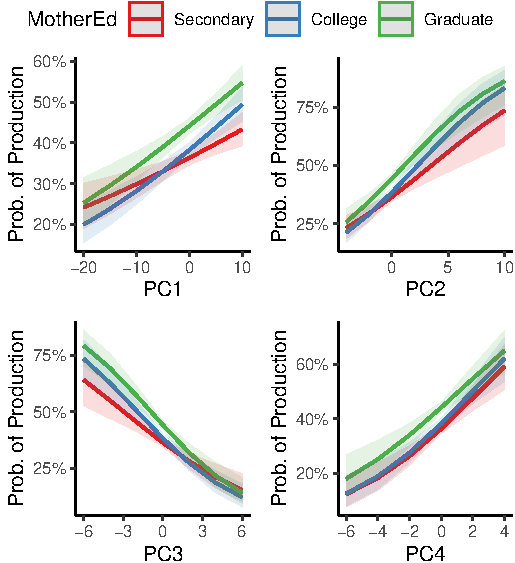
\includegraphics{figs/unnamed-chunk-9-1} 

}

\caption[Significant regression coefficients for predicting CDI AoAs with PCs and lexical class for English (top) and French (bottom)]{Significant regression coefficients for predicting CDI AoAs with PCs and lexical class for English (top) and French (bottom). Abbreviated levels of lexical class (LC) are function words (`func'), adjectives (`adj'), and 'other' includes items refering to games, routines, and people.}\label{fig:unnamed-chunk-9}
\end{figure}
\end{CodeChunk}

\hypertarget{principal-components-and-maternal-education-q3}{%
\subsection{Principal components and maternal education
(Q3)}\label{principal-components-and-maternal-education-q3}}

Correlations between parental SES and children's language development
are documented in a large body of literature, and SES seems to be
predictive of aspects of word learning (Hoff, 2003). Previous findings
also relate SES status to book reading (Shen \& Del Tufo, 2022), which
in turn seems to be related to better language skills (Bus, Van
Ijzendoorn, \& Pellegrini, 1995; Sénéchal \& LeFevre, 2002). These
findings suggest that the vocabulary composition of children whose
mothers are highly-educated (parental education being a proxy for
household SES) may be better predicted by the word frequencies seen in
child-directed books, rather than those from child-directed speech. To
test this idea, we fit a series of exploratory logistic regressions
successively adding the PCs to predict the number of children in
Wordbank who produce or don't produce each item. Due to lack of maternal
education data for French data, we focused on American English-learning
children. We included interactions of mother's education and children's
age with each PC; interactions of this type indicate that a particular
type of register or source might be more important to acquisition for
one SES group or another.

American English data from Wordbank contained 2,776 CDI:WS
administrations with mother's education dichotomously coded (N=1160 with
at most some college education; N=1616 with a college degree or more).
The series of ANOVAs indicated that PC1 through PC5 significantly
improved the model fits, but that adding PC6 was not justified. Thus, we
analyzed the model that included the first five PCs. This model showed
significant main effects of age, mother's education, and all five PCs
(all \(p<.001\)). Faster learning was predicted for words with higher
values on PC1 (overall frequency; \(\beta=.10\)), PC2 (child-directed
speech; \(\beta=.45\)), and PC4 (media vs.~books; \(\beta=.28\)). Slower
learning was predicted for words with higher values on PC3
(\(\beta=-.34\)) or PC5 (\(\beta=-.49\)). There was a significant
positive interaction of age with mother's education (\(\beta=.06\),
\(p<.001\)), shown in Figure 3. There were also significant interactions
of age and all five PCs, although the coefficients were all of a small
magnitude (\(\beta\)s \textless{} .01).

In the critical test of our hypothesis, PC1 and PC5 interacted
significantly with mother's education. Shown in Figure 3, children of
higher-educated mothers were more likely to know words that were higher
on PC1 (overall frequency; \(\beta = .03\), \(p<.001\)), while they were
less likely to know words that were high on PC5 (\(\beta = -.09\),
\(p=.01\)). Words more frequent in child-directed speech are high on
PC5, while words that are more often in child-directed books are low on
PC5, meaning that this interaction indicates children with
higher-educated mothers are more likely to learn words that occur in
books (rather than words that occur in speech). As seen in Table 4,
these include animal sounds, which occur frequently in baby books and in
other analyses tend to be known more by children whose mothers have more
education (Frank, Braginsky, Yurovsky, \& Marchman, 2021).

\begin{CodeChunk}
\begin{table}

\caption{\label{tab:unnamed-chunk-10}Top 5 words with improved prediction of AoA when adding each PC for English (EN) and French (FR)}
\centering
\begin{tabular}[t]{cc}
\toprule
Lang PC & Top 5 Words\\
\midrule
\cellcolor{gray!6}{EN +1} & \cellcolor{gray!6}{can, no, cockadoodledoo, now, time}\\
EN +2 & yes, gas, don't, uhoh, no\\
\cellcolor{gray!6}{EN +3} & \cellcolor{gray!6}{camping, bye, jeans, smile, babysitter}\\
EN +4 & was, lot, lips, gonna, hafta\\
\cellcolor{gray!6}{EN +5} & \cellcolor{gray!6}{mommy, grrr, cockadoodledoo, tissue, babysitter}\\
EN +6 & would, mine, does, my, could\\
\cellcolor{gray!6}{FR +1} & \cellcolor{gray!6}{\makecell[l]{le, faire, au sommet de, au sujet de, lequel \\ (EN: the, do, on top, about, which)}}\\
FR +2 & \makecell[c]{coincé, sombre, maître, oui, aïe \\ (EN: stuck, dark, teacher, yes, ouch)}\\
\bottomrule
\end{tabular}
\end{table}

\end{CodeChunk}

\hypertarget{general-discussion}{%
\section{General Discussion}\label{general-discussion}}

We investigated how linguistic input varies across the types of language
that children may experience using word frequency distributions garnered
from child-directed and adult-directed corpora of speech, books, and
media (TV and movies). Since frequencies are highly correlated, we found
the principal components (PCs) of these distributions, which revealed
systematic variation along source and register dimensions. Most
variation in frequency is shared across all the different sources and
registers in our study. French in particular showed high correlations,
perhaps due to smaller corpus size or due to noise introduced by
stemming and lemmatization. In spite of this, other PCs in both
languages picked up on consistent differences in both register and
source. In English, child-directed speech captured a substantial part of
the variance as a second principal component, suggesting real
differences in word frequencies in this register. In French, in
contrast, child-directed speech loaded strongly on the third principal
component, while the second component picked up on bookish words (both
child- and adult-directed) -- a distinction captured by a smaller PC for
English.

\begin{CodeChunk}
\begin{figure}[t]

{\centering 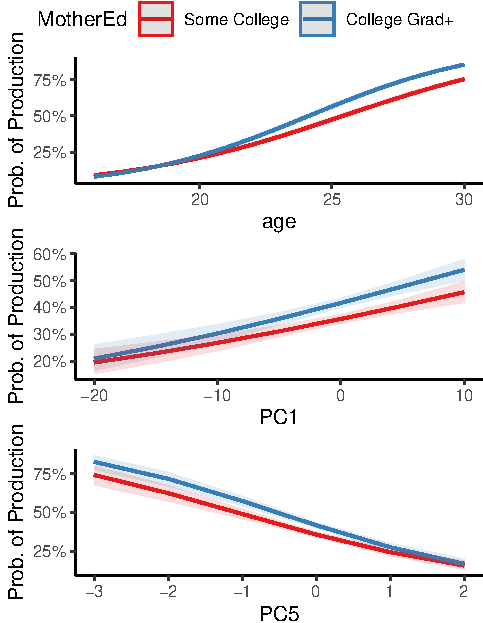
\includegraphics{figs/unnamed-chunk-12-1} 

}

\caption[Predicted effects on the probability of English-speaking children producing CDI:WS words based on maternal education]{Predicted effects on the probability of English-speaking children producing CDI:WS words based on maternal education. A significant positive interaction with age (top) shows an increasing effect of maternal education as children age. A significant positive interaction with PC1 (middle) shows that words with higher overall frequency are produced more by children with more educated mothers. A negative interaction with PC5 shows that children with more educated mothers are likely to produce words more representative of child-directed books, rather than child-directed speech.}\label{fig:unnamed-chunk-12}
\end{figure}
\end{CodeChunk}

Multiple components were predictive of children's age of acquisition of
words from the CDI, especially for English. Child-directed speech,
adult-directed speech, but also books and media were all relevant in
predicting age of acquisition. In French, the component distinguishing
books and speech was most relevant in predicting age of acquisition.
Lending some qualitative support to these conclusions, the specific
words that were improved by the addition of particular PCs appeared
somewhat related to these sources and registers.

We also used English Wordbank data to test how well frequency components
combine with mother's education to predict children's early word
learning. This exploratory analysis revealed significant contributions
of the first five PCs, as well as interactions of mother's education
with PC1 (overall frequency) and PC5 (child-directed speech vs.~books).
This intriguing finding suggests that the early language advantage shown
by children of more highly-educated mothers (and thus in higher-SES
households; cf.~Hoff, 2003) may in part be due to greater amounts of
shared reading time. A target for future research is to predict
individual children's learning of particular words using these principal
components, in combination with measures of how much time their child
spends receiving input from each input source ({[}adult-
vs.~child-directed{]} x {[}books, media, speech{]}).

This research has a number of limitations that point the way to future
work. First, our study is an observational linkage between frequencies
as estimated from one set of materials and acquisition trajectories from
wholly different children. We expect that frequencies represent
estimates of an average experience by a member of a particular
linguistic or cultural group, but they are certainly biased by their
specific source. Second, corpora of different sizes represent the
sources and registers for each language, and less data were available
overall for French. Observed differences between the two languages could
thus be partly attributed to differences in corpus size and sources. For
example, the French corpora are composed of several smaller ones, due to
the lack of large accessible corpora, and have slightly different
makeup, e.g.~short stories in French vs.~longer books in English. Third,
most English and some French child-directed books where published
decades ago, and are used due to the lack of available open-source
contemporary books. This could yield different frequency distributions,
however this difference should be negligible for the specific CDI words
tested here. Moreover, we note the difficulty of drawing conclusions
about these results, since the conclusions are based on interpretations
of the relevant dimensions of the different principal components.
Finally, although an effort was made to examine two languages, French
and English represent only a tiny subset of the broader set of
linguistic environments in which children acquire their vocabulary. In
sum, by better understanding the similarity and differences between word
frequencies that children experience in different contexts, future
research in this vein holds the promise to predict individual
differences in children's early word learning on the basis of their
daily routines.

\hypertarget{acknowledgements}{%
\section{Acknowledgements}\label{acknowledgements}}

This research was supported by the Stanford Maternal and Child Health
Research Institute, and funded in part by the Fyssen Foundation. We
thank members of the Language and Cognition lab for their feedback.

\hypertarget{references}{%
\section{References}\label{references}}

\setlength{\parindent}{-0.1in} 
\setlength{\leftskip}{0.125in}

\noindent

\hypertarget{refs}{}
\leavevmode\hypertarget{ref-ambridge2015ubiquity}{}%
Ambridge, B., Kidd, E., Rowland, C. F., \& Theakston, A. L. (2015). The
ubiquity of frequency effects in first language acquisition.
\emph{Journal of Child Language}, \emph{42}(2), 239--273.

\leavevmode\hypertarget{ref-andre2010mise}{}%
André, V., \& Canut, E. (2010). Mise à disposition de corpus oraux
interactifs: Le projet tcof (traitement de corpus oraux en français).
\emph{Pratiques. Linguistique, Littérature, Didactique}, (147-148),
35--51.

\leavevmode\hypertarget{ref-balthasar2005plateforme}{}%
Balthasar, L., \& Bert, M. (2005). La plateforme corpus de langues
parlées en interaction(CLAPI). Historique, état des lieux, perspectives.
\emph{Lidil. Revue de Linguistique et de Didactique Des Langues}, (31),
13--33.

\leavevmode\hypertarget{ref-braginsky2019consistency}{}%
Braginsky, M., Yurovsky, D., Marchman, V. A., \& Frank, M. C. (2019).
Consistency and variability in children's word learning across
languages. \emph{Open Mind}, \emph{3}, 52--67.

\leavevmode\hypertarget{ref-branca2012discours}{}%
Branca-Rosoff, S., Fleury, S., Lefeuvre, F., \& Pires, M. (2012).
Discours sur la ville. Présentation du corpus de français parlé parisien
des années 2000 (cfpp2000). \emph{Article En Ligne, Http://Cfpp2000.
Univparis3. Fr/Articles. Html}.

\leavevmode\hypertarget{ref-bus1995joint}{}%
Bus, A. G., Van Ijzendoorn, M. H., \& Pellegrini, A. D. (1995). Joint
book reading makes for success in learning to read: A meta-analysis on
intergenerational transmission of literacy. \emph{Review of Educational
Research}, \emph{65}(1), 1--21.

\leavevmode\hypertarget{ref-charlesworth2021gender}{}%
Charlesworth, T. E., Yang, V., Mann, T. C., Kurdi, B., \& Banaji, M. R.
(2021). Gender stereotypes in natural language: Word embeddings show
robust consistency across child and adult language corpora of more than
65 million words. \emph{Psychological Science}, \emph{32}(2), 218--240.

\leavevmode\hypertarget{ref-dawson2021features}{}%
Dawson, N., Hsiao, Y., Wei Ming Tan, A., Banerji, N., \& Nation, K.
(2021). Features of lexical richness in children's books: Comparisons
with child-directed speech. \emph{Language Development Research}.

\leavevmode\hypertarget{ref-dodge2008concise}{}%
Dodge, Y. (2008). \emph{The concise encyclopedia of statistics}.
Springer Science \& Business Media.

\leavevmode\hypertarget{ref-fenson1994variability}{}%
Fenson, L., Dale, P. S., Reznick, J. S., Bates, E., Thal, D. J.,
Pethick, S. J., \ldots{} Stiles, J. (1994). Variability in early
communicative development. \emph{Monographs of the Society for Research
in Child Development}, i--185.

\leavevmode\hypertarget{ref-fenson2007}{}%
Fenson, L., Marchman, V. A., Thal, D. J., Dale, P. S., Reznick, J. S.,
\& Bates, E. (2007). \emph{MacArthur-Bates Communicative Development
Inventories: User's guide and technical manual (2nd ed.)}. Baltimore,
MD: Brookes.

\leavevmode\hypertarget{ref-fernald2013ses}{}%
Fernald, A., Marchman, V. A., \& Weisleder, A. (2013). SES differences
in language processing skill and vocabulary are evident at 18 months.
\emph{Developmental Science}, \emph{16}(2), 234--248.

\leavevmode\hypertarget{ref-frank2017wordbank}{}%
Frank, M. C., Braginsky, M., Yurovsky, D., \& Marchman, V. A. (2017).
Wordbank: An open repository for developmental vocabulary data.
\emph{Journal of Child Language}, \emph{44}(3), 677--694.

\leavevmode\hypertarget{ref-frank2021}{}%
Frank, M. C., Braginsky, M., Yurovsky, D., \& Marchman, V. A. (2021).
\emph{Variability and consistency in early language learning: The
wordbank project}. MIT Press.

\leavevmode\hypertarget{ref-godfrey1993switchboard}{}%
Godfrey, J., \& Holliman, E. (1993). Switchboard-1 release 2 ldc97s62.
\emph{Linguistic Data Consortium}.

\leavevmode\hypertarget{ref-golinkoff2015baby}{}%
Golinkoff, R. M., Can, D. D., Soderstrom, M., \& Hirsh-Pasek, K. (2015).
(Baby) talk to me: The social context of infant-directed speech and its
effects on early language acquisition. \emph{Current Directions in
Psychological Science}, \emph{24}(5), 339--344.

\leavevmode\hypertarget{ref-goodman2008}{}%
Goodman, J. C., Dale, P. S., \& Li, P. (2008). Does frequency count?
Parental input and the acquisition of vocabulary. \emph{Journal of Child
Language}, \emph{35}(3), 515--531.

\leavevmode\hypertarget{ref-hart1995meaningful}{}%
Hart, B., \& Risley, T. R. (1995). \emph{Meaningful differences in the
everyday experience of young american children.} Paul H Brookes
Publishing.

\leavevmode\hypertarget{ref-hill2015goldilocks}{}%
Hill, F., Bordes, A., Chopra, S., \& Weston, J. (2015). The goldilocks
principle: Reading children's books with explicit memory
representations. \emph{arXiv Preprint arXiv:1511.02301}.

\leavevmode\hypertarget{ref-hoff2003specificity}{}%
Hoff, E. (2003). The specificity of environmental influence:
Socioeconomic status affects early vocabulary development via maternal
speech. \emph{Child Development}, \emph{74}(5), 1368--1378.

\leavevmode\hypertarget{ref-macwhinney2000childes}{}%
MacWhinney, B. (2000). \emph{The childes project: Tools for analyzing
talk. Transcription format and programs} (Vol. 1). Psychology Press.

\leavevmode\hypertarget{ref-montag2015words}{}%
Montag, J. L., Jones, M. N., \& Smith, L. B. (2015). The words children
hear: Picture books and the statistics for language learning.
\emph{Psychological Science}, \emph{26}(9), 1489--1496.

\leavevmode\hypertarget{ref-porter2001snowball}{}%
Porter, M. F. (2001). Snowball: A language for stemming algorithms.

\leavevmode\hypertarget{ref-rowe2012longitudinal}{}%
Rowe, M. L. (2012). A longitudinal investigation of the role of quantity
and quality of child-directed speech in vocabulary development.
\emph{Child Development}, \emph{83}(5), 1762--1774.

\leavevmode\hypertarget{ref-rowe2018understanding}{}%
Rowe, M. L. (2018). Understanding socioeconomic differences in parents'
speech to children. \emph{Child Development Perspectives}, \emph{12}(2),
122--127.

\leavevmode\hypertarget{ref-senechal2002parental}{}%
Sénéchal, M., \& LeFevre, J.-A. (2002). Parental involvement in the
development of children's reading skill: A five-year longitudinal study.
\emph{Child Development}, \emph{73}(2), 445--460.

\leavevmode\hypertarget{ref-shen2022parent}{}%
Shen, Y., \& Del Tufo, S. N. (2022). Parent-child shared book reading
mediates the impact of socioeconomic status on heritage language
learners' emergent literacy. \emph{Early Childhood Research Quarterly},
\emph{59}, 254--264.

\leavevmode\hypertarget{ref-soderstrom2007beyond}{}%
Soderstrom, M. (2007). Beyond babytalk: Re-evaluating the nature and
content of speech input to preverbal infants. \emph{Developmental
Review}, \emph{27}(4), 501--532.

\bibliographystyle{apacite}


\end{document}
